For viewing the conveyor belt system, it is of course important that the user is able to see the properties of every conveyor belt clearly. That is, the following three properties should be visible:
\begin{itemize}
  \item the \textit{shape} (is it horizontal, ascending\,/\,descending or a bend);
  \item the \textit{orientation} (is the conveyor belt oriented in the $x$- or the $y$-direction);
  \item the \textit{direction} (towards which of the two possible directions does it move).
\end{itemize}
The first two properties do not need a lot of realism: only a rough approximation of the shape will suffice for that. However, for the user to be able to see the direction, just the drawn shape will not be enough.

In the building mode, we can simply draw arrows on top of the conveyor belts that indicate the direction. During the simulation however, we think that looks very bad. Instead, we want the conveyor belts to look like they really move. To do this in an easy way, we can use a texture on the surface of the conveyor belt, and animate its texture coordinates.

We can use a texture of a small part of the conveyor belt, and repeat it in the length direction of the belt. A requirement is then that the texture does not get deformed, that is, the texture coordinates should be such that every repetition of the texture has (about) the same size. This is especially important since we are going to animate the texture, meaning that deformations in the texture would become visible as stretching or shortening of parts of the conveyor belt.

\subsubsection{Calculating texture coordinates}
First note that only the texture coordinates in the length direction are important here; for the other direction we can just use $0$ for the left side and $1$ for the right side.

Now, for calculating the texture coordinates, we use the following strategy: we use fixed values for every point at the conveyor belt, and then we animate those linearly. Assuming that the fixed values indeed do not deform the texture too much, the animated texture will also not be deformed in this way.

The problem left now is determining the fixed values. We pose the following requirements for them.
\begin{itemize}
  \item As said before, they should not deform the texture (or only a little bit). Said differently, there is some $r$ such that for every point $p$ on the belt,
  \[
    l(p) \approx r \cdot t(p),
  \]
  where $l(p)$ means the length of the belt until point $p$ and $t(p)$ denotes the texture coordinate at point $p$.
  \item Furthermore, we want the blocks to be tileable. As described in section~\ref{subsubsec:drawing-adjacent}, we want to draw adjacent blocks as one large conveyor belt. Therefore, we require that $t(p) \in \mathbb{Z}$ for points $p$ that connect to other belts.
  \item Finally, we do not want the texture coordinates to become very high, since that means that the texture will be repeated many times on the conveyor belt, which may become noticable.
\end{itemize}
We tried to find an exact solution, but this turns out to be hard, especially since the requirements are quite vague. Finally, we came up with an approximate solution manually, that is shown in Figure~\ref{fig:sketch-texturing}.
\begin{figure}
  \begin{center}
    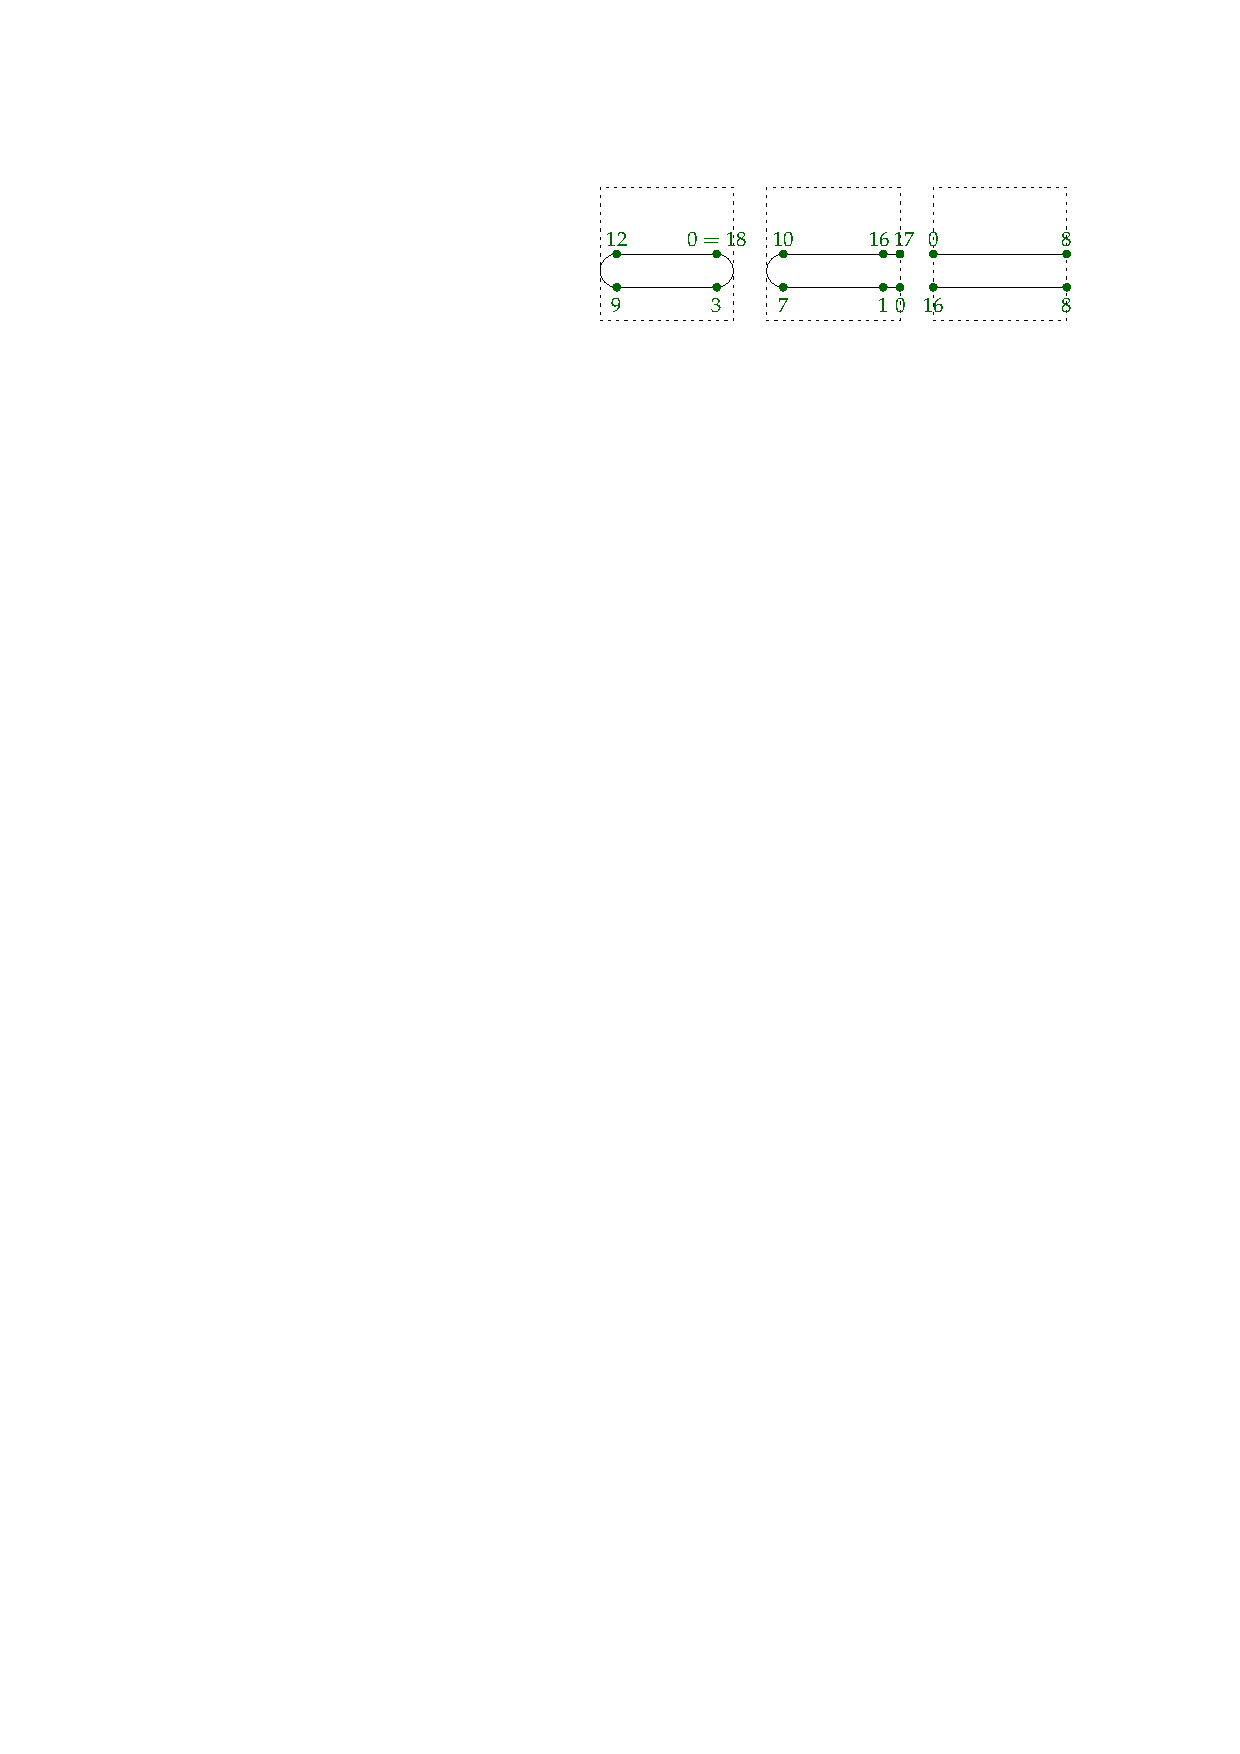
\includegraphics{sketch-texturing}
    \caption{Texture coordinates for the horizontal conveyor belt.}
    \label{fig:sketch-texturing}
  \end{center}
\end{figure}

\subsubsection{Drawing adjacent conveyor belts}
\label{subsubsec:drawing-adjacent}
When two conveyor belts are adjacent to each other, they should be drawn as one large belt. (This makes sense, since probably in real systems also one long belt would be used instead of many short ones.) See Figure~\ref{fig:blocks-adjacent} for a sketch.
\begin{figure}
  \begin{center}
    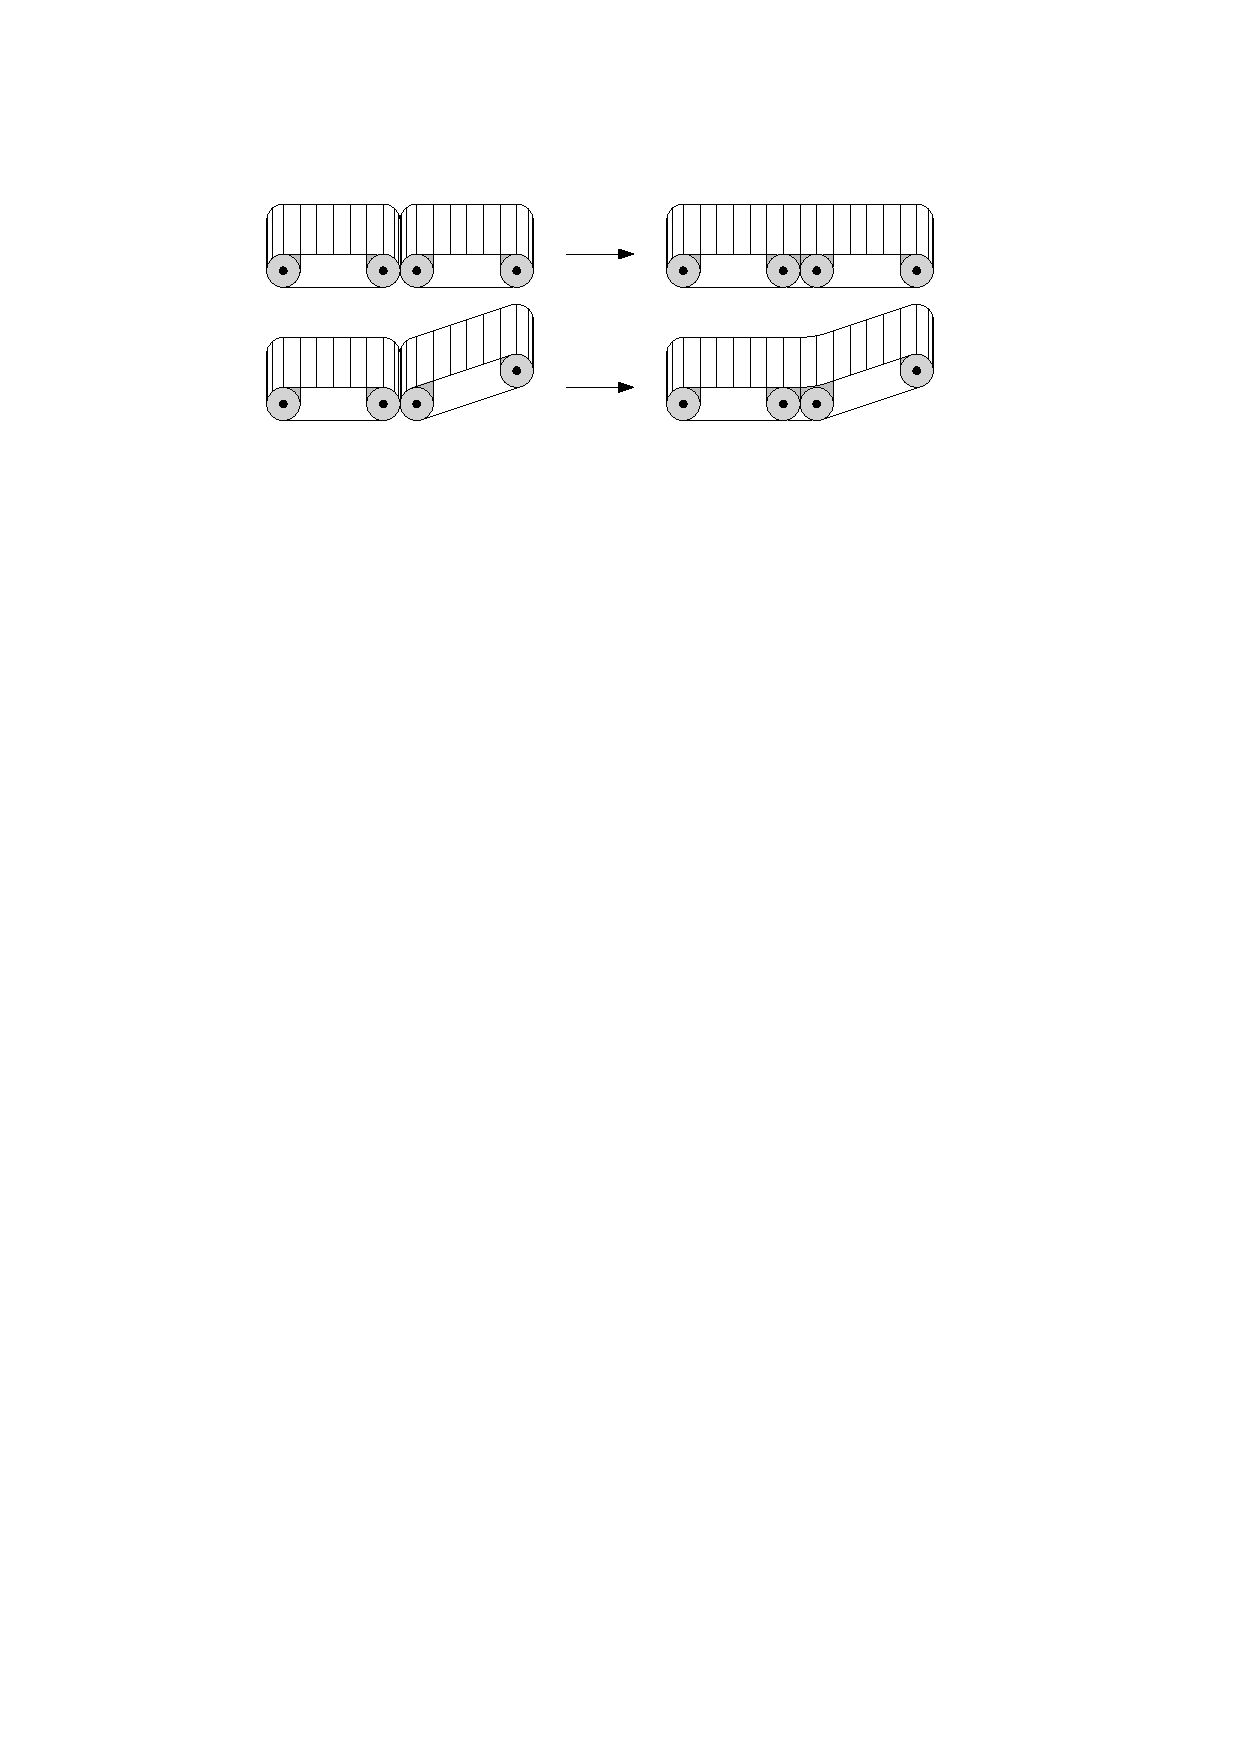
\includegraphics{blocks-adjacent}
    \caption{Adjacent blocks should be drawn together.}
    \label{fig:blocks-adjacent}
  \end{center}
\end{figure}

This is not only a feature for realism, but it also is an additional clue for the user to view the conveyor belt system easier. Namely, when one large belt is shown, the user can be sure that the belts are correctly adjacent to each other and that they all have the same direction.
